\documentclass[../../main.tex]{subfiles}

\begin{document}

\section{Experimento 3: 45 períodos observados, 5 de dependencia} \label{sec:exp3} 
Aquí redujimos aún más la cantidad de períodos de dependencia, pasando de 10 a 5, pero
esta vez con 0 incrementos. Esto implica que la proporción de períodos de dependencia
sobre observados es de 0.11, pero la tendencia modelada en ellos es monótona decreciente,
como se observa en la Figura \ref{fig:time_series_exp3}. Nuevamente, tomamos
\(\mu_{{EF}_{NiNi}} = 10\).

\begin{figure}[ht]
    \centering
    \begin{minipage}{0.48\textwidth}
        \centering
        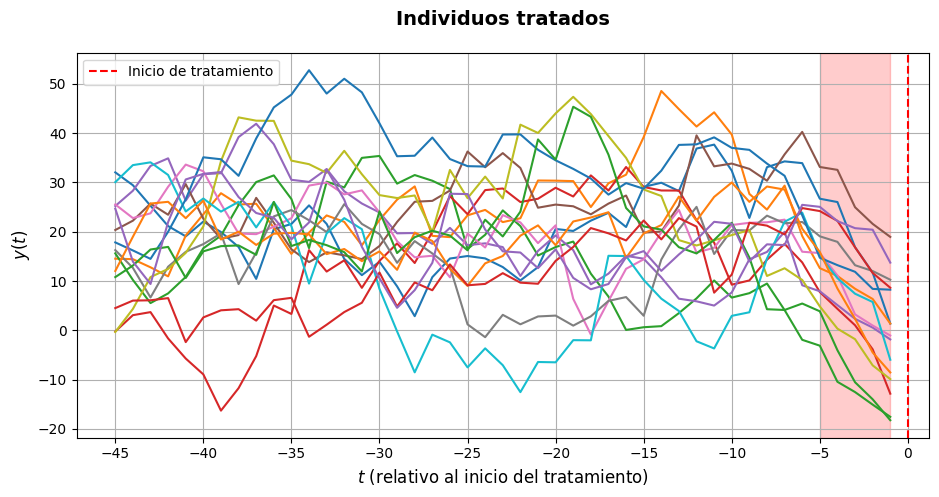
\includegraphics[scale=0.3]{figs/Exp3/tratados_sim63.png}
    \end{minipage}
    \hfill
    \begin{minipage}{0.48\textwidth}
        \centering
        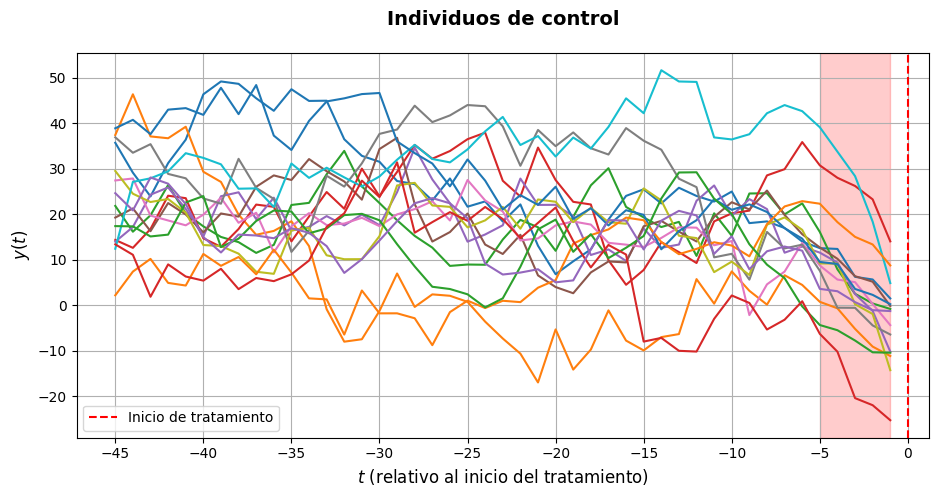
\includegraphics[scale=0.3]{figs/Exp3/controles_sim63.png}
    \end{minipage}
    \vspace{0.5em}
    \begin{minipage}{0.6\textwidth}
        \centering
        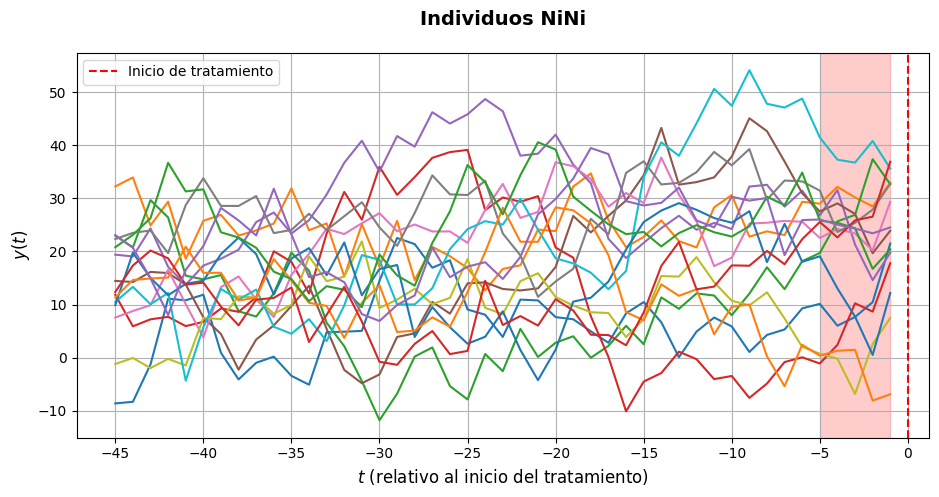
\includegraphics[scale=0.3]{figs/Exp3/ninis_sim63.png}
    \end{minipage}
    \caption{Ejemplos de series de tiempo generadas para cada grupo en el experimento 3.
    Los períodos con un fondo rojo indican los períodos de dependencia para tratados y
    controles, en donde se ve el comportamiento monótono decreciente. La línea
    punteada roja indica el inicio de tratamiento para cada individuo.}
    \label{fig:time_series_exp3}
\end{figure}

La Tabla \ref{tab:results_exp3} muestra los valores obtenidos de las diferentes métricas.
Para nuestra sorpresa, en el caso de las redes, fueron bastante similares - y hasta en
algunos casos mejores - que los obtenidos en el \hyperref[sec:exp1]{experimento 1}, en
donde teníamos la misma cantidad de períodos observados, de los cuales casi la mitad
mostraban un compartamiento decreciente con ruido. Esto parece indicar que quitar los
incrementos en los períodos de dependencia, lo cual disminuye la complejidad del patrón a
hallar, favorece en gran medida a las redes neuronales. Sin embargo, el PSM presentó un
rendimiento menor al visto en dicho escenario, contrario a nuestra hipótesis.

\begin{table}[ht]
    \centering
    \renewcommand{\arraystretch}{1.2}
    \begin{tabular}{|c|c|c|c|}
        \hline
         & \textbf{Puntaje} \(F_1\) & \textbf{Precisión} & \textbf{Recuperación} \\ \hline\hline
        \textbf{LSTM}
            & $0.82570 \pm 0.01856$ & $0.72740 \pm 0.03211$ & $0.95680 \pm 0.02282$ \\ \hline
        \textbf{Convolucional}
            & $0.84641 \pm 0.01741$ & $0.75091 \pm 0.03095$ & $\mathbf{0.97133 \pm 0.01503}$ \\ \hline
        \makecell{\textbf{LSTM +} \\ \textbf{Convolucional}}
            & $\mathbf{0.84759 \pm 0.01555}$ & $\mathbf{0.75319 \pm 0.02809}$ & $0.97040 \pm 0.01510$ \\ \hline
        \textbf{PSM}
            & $0.53324 \pm 0.01634$ & $0.53398 \pm 0.01638$ & $0.53251 \pm 0.01633$ \\
        \hline
    \end{tabular}
    \caption{Promedio de las métricas \(F_1\), precisión y sensibilidad sobre la
    clase positiva (controles) en el conjunto de test en las 100 simulaciones del
    experimento 3.}
    \label{tab:results_exp3}
\end{table}

En la Tabla \ref{tab:hyperparams_exp3} se reflejan los resultados correspondientes
a los hiperparámetros, en donde nuevamente se observa lo mismo que antes.

\begin{table}[H]
    \centering
    \renewcommand{\arraystretch}{1.2}
    \begin{tabular}{|c|c|c|c|c|}
        \hline
            & \makecell{\textbf{Tamaño}\\\textbf{de lote}}
            & \makecell{\textbf{Neuronas en}\\\textbf{capas ocultas}}
            & \makecell{\textbf{Tasa de}\\\textbf{aprendizaje}}
            & \textbf{Dropout} \\ \hline\hline
        \textbf{LSTM}
            & 64 (35\%) & 128 (57\%) & 0.001 (100\%) & 0.3 (64\%) \\ \hline
        \textbf{Convolucional}
            & 32 (42\%) & -          & 0.001 (89\%)  & 0.3 (76\%) \\ \hline
        \makecell{\textbf{LSTM +}\\\textbf{Convolucional}}
            & 32 (50\%) & 32 (35\%), 64 (35\%) & 0.001 (87\%) & 0.3 (71\%) \\
        \hline
    \end{tabular}
    \caption{Valores de hiperparámetros seleccionados con mayor frecuencia en las 100
    simulaciones en cada arquitectura en el experimento 3. Cada celda contiene dicho valor
    y entre paréntesis el porcentaje de simulaciones en el resultó ser el mejor, de
    acuerdo a la optimización realizada por Optuna mediante validación cruzada.}
    \label{tab:hyperparams_exp3}
\end{table}

\end{document}